% \begin{frame}
% \frametitle{Modélisation des réseaux de régulation biologique}
% 
% \begin{itemize}
%  \item 
%  \item 
% \end{itemize}
%\end{frame}

\begin{frame}
\frametitle{Modélisation discrètes}

\begin{itemize}
 \item Chaque composant possède un nombre fini de \tval{niveaux qualitatifs} (\{0,1,2,...\}).
 \item Fonctions donnant le \tval{niveau suivant l'état des régulateurs.}
\end{itemize}
\bigskip
\begin{tikzpicture}
 \node[scale=1] (brn) at (0,5) {\begin{tikzpicture}[grn]
      \path[use as bounding box] (-0.3,-0.75) rectangle (4,.75);
      \node[inner sep=0] (b) at (2,0) {b};
      \node[inner sep=0] (a) at (0,0) {a};
            
      \node[elabel, below=-.8em of a] {$0..2$};
      \node[elabel, below=-.8em of b] {$0..1$};
     
      
      \path[->]
        (a) edge[loop above] node[elabel, above=-5pt] {$+2$}
        (a) edge[bend right] node[elabel, below=-5pt] {$+1$} (b)
        (b) edge[bend right] node[elabel, above=-5pt] {$-1$} (a);
    \end{tikzpicture}};
 
\node (plus) at (-1,3.5) {\textbf{+}};
    
\node (ft) at (-1,3) {Fonction de transition};

\node[auto] (sg) at (6,4) {
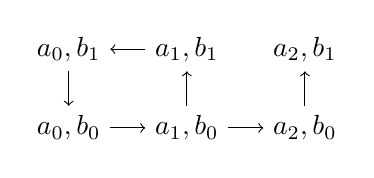
\begin{tikzpicture}[node distance=1.5cm]
  \node (s01) {$\RRBetat{a_0,b_1}$};
  \node[right of=s01] (s11) {$\RRBetat{a_1,b_1}$};
  \node[right of=s11] (s21) {$\RRBetat{a_2,b_1}$};
  \node[below of=s01, node distance=1cm] (s00) {$\RRBetat{a_0,b_0}$};
  \node[right of=s00] (s10) {$\RRBetat{a_1,b_0}$};
  \node[right of=s10] (s20) {$\RRBetat{a_2,b_0}$};
  \path[->]
    (s01) edge (s00)
    (s00) edge (s10)
    (s10) edge (s11)
    (s11) edge (s01)
    (s10) edge (s20)
    (s20) edge (s21)
  ;
\end{tikzpicture}};
%\node[scale=0.6] (sg) at (2,1) {
\begin{tikzpicture}[line join=bevel,font=\LARGE]
%%
  \node (6) at (405.0bp,18.0bp) [reach,nd4] {$\langle a_2,b_1,c_0\rangle$};
  \node (2) at (405.0bp,90.0bp) [reach,nd3] {$\langle a_2,b_0,c_0\rangle$};
  \node (1) at (570.0bp,90.0bp) [reach,nd1] {$\langle a_1,b_0,c_0\rangle$};
  \node (0) at (469.0bp,162.0bp) [reach,nd0] {$s_0 = \langle a_0,b_0,c_0\rangle$};
  \node (4) at (469.0bp,234.0bp) [reach,nd5] {$\langle a_0,b_1,c_0\rangle$};
 
 
  \draw [->,arc3] (0) ..controls (445.65bp,135.46bp) and (435.95bp,124.86bp)  .. (2);
  \draw [->,arc5] (0) ..controls (475.71bp,188.03bp) and (475.94bp,197.36bp)  .. (4);
  \draw [->,arc4] (2) ..controls (405.0bp,63.983bp) and (405.0bp,54.712bp)  .. (6);
  \draw [->,arc1] (0) ..controls (499.93bp,134.79bp) and (517.41bp,122.58bp)  .. (1);
  \draw [->,arc2] (1) ..controls (539.0bp,117.26bp) and (521.52bp,129.47bp)  .. (0);
  \draw [->,arc5] (4) ..controls (462.3bp,208.35bp) and (462.06bp,199.03bp)  .. (0);
 
%
\end{tikzpicture}

};
\path 
(2,4) edge[->,line width=6pt, color=lightgray] (sg)
;
\end{tikzpicture}

\begin{center}
 {\small \color{darkgreen} [\citekauffman]}\\
 {\small \color{darkgreen} [\citethomas]}
\end{center}

\end{frame}


\begin{frame}
\frametitle{Modélisation hybride}
\framesubtitle{\'Etats discrets et transitions caractéristiques hybrides}

\tval{Introduction de l'aléatoire et du temps pour les transitions}\\
\medskip
\textbf{Modèles stochastiques} \\
Variables aléatoires généralement exponentielles. 
\begin{itemize}
 \item $\pi$-calcul stochastique. 
 \item Réseaux de Petri stochastiques.
\end{itemize}
% \begin{center}
% {\small \color{darkgreen} [\citestocha]}\\
%  
% \end{center}


\bigskip

\textbf{Modèles temporisés}
\begin{itemize}
 \item Automates temporisés / hybrides.
 \item Réseaux de Petri temporisés.
\end{itemize}

\medskip

\textbf{Frappes de processus}.
% \begin{center}
% {\small \color{darkgreen} [\citetemp]}\\
% 
% \end{center}


%nécessité d'estimer les paramètre à partir des données 

\end{frame}

